% !TEX root = ./main.tex
% !TEX encoding = UTF-8 Unicode
% !TEX program = pdflatex
% !TeX spellcheck = it_IT

\chapter{PCA e Clustering}
Estrapolare un Workload sintetico a partire dal workload reale riportato nel file
 \textit{PCA-CLASTERING-2017.jmp}.

\section{Obiettivo}
A partire dal workload reale, si vuole ottenere un \textbf{workload sintetico},
caratterizzato da un numero di osservazioni minori, che conservi quanta
più varianza possibile.

\section{Estrazione del Workload Sintetico}
Per estrarre il workload sintetico, dopo aver visionato i dati, si è scelto
di seguire il seguente procedimento:

\begin{itemize}
  \item Analisi del \textbf{\textit{CV(Coefficiente di Variazione)}} per
  eliminare i parametri statisticamente non significativi;
  \item \textbf{\textit{PCA(Principal Component Analysis)}} per ridurre il
  numero di parametri e per eliminare la correlazione tra essi;
  \item \textbf{\textit{Clustering}} per ridurre il numero di esperimenti.
\end{itemize}


\subsection{Analisi del Coefficiente di Variazione}
In prima istanza, è stata effettuata un'analisi sul coefficiente di variazione(CV),
il quale esprime la dispersione dei valori dei singoli parametri attorno alla loro media.\\
Quando il coefficiente di variazione è troppo piccolo (in questo caso 0), il parametro
corrispondente non è statisticamente significativo e quindi è possibile eliminarlo.\\
Nella figura si nota che non ci sono colonne con coefficiente di variazione nullo,
quindi tutti i parametri saranno utilizzati nelle successive analisi.

\begin{figure}[!htbp]
	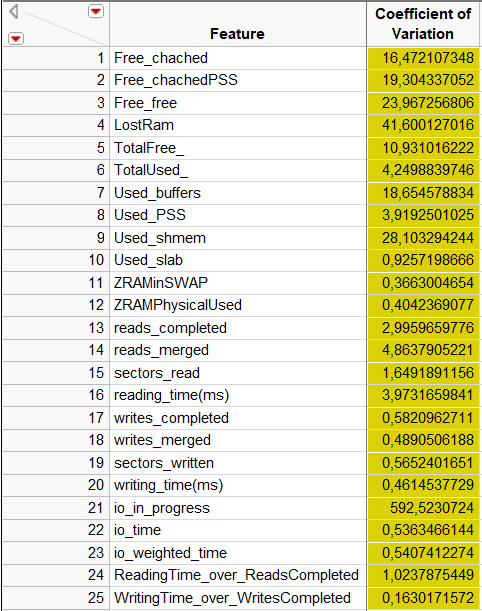
\includegraphics[width=.7\linewidth,keepaspectratio]{cov.png}
  \caption{Coefficiente di Variazione(CV)}
  \label{}
\end{figure}

\subsection{PCA}
In questa fase è stata applicata la
\textbf{\textit{PCA(Principal Component Analysis)}}
la quale trasforma un workload con parametri correlati in uno contente parametri
non correlati, ottenuti come combinazione lineare, pesata, dei parametri iniziali.\\
L'utilizzo della PCA è fondamentale anche per la successiva fase di clustering, in
quanto quest'ultimo funziona meglio quando i parametri sono incorrelati.\\
Per effettuare la PCA si è fatto utilizzo del tool statistico \textit{\textbf{JMP}}, nella
\figurename~\ref{pca} è riportato l'output.\\

\begin{figure}[!htbp]
	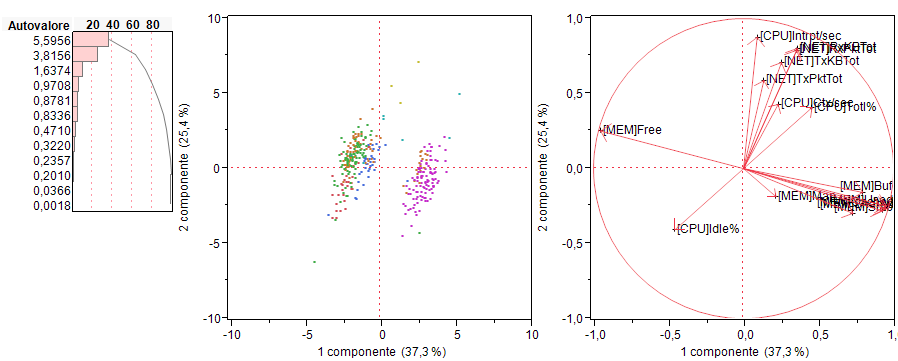
\includegraphics[width=\linewidth,keepaspectratio]{pca.png}
  \caption{Risultato PCA}
  \label{pca}
\end{figure}

\begin{figure}[!htbp]
	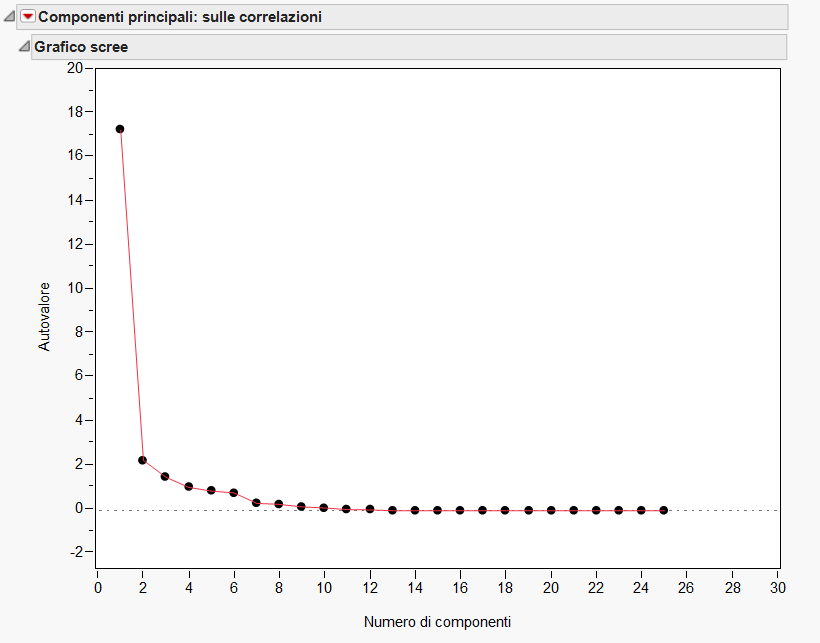
\includegraphics[width=\linewidth,keepaspectratio]{grafico_scree.png}
  \caption{Grafico Scree}
  \label{grafico_scree}
\end{figure}

A partire dalla \figurename~\ref{grafico_scree}, rappresentante
sull'asse delle x il numero di componenti principali e sull'asse delle y
gli autovalori, per scegliere il numero di componenti principali, si considera
il ginocchio della curva.\\
In quel punto si è sicuri che aggiungendo un'ulteriore componente la varianza
conservata non aumenta significativamente.\\
Quindi si è scelto di considerare 6 componenti principali.\\

\begin{figure}[!htbp]
	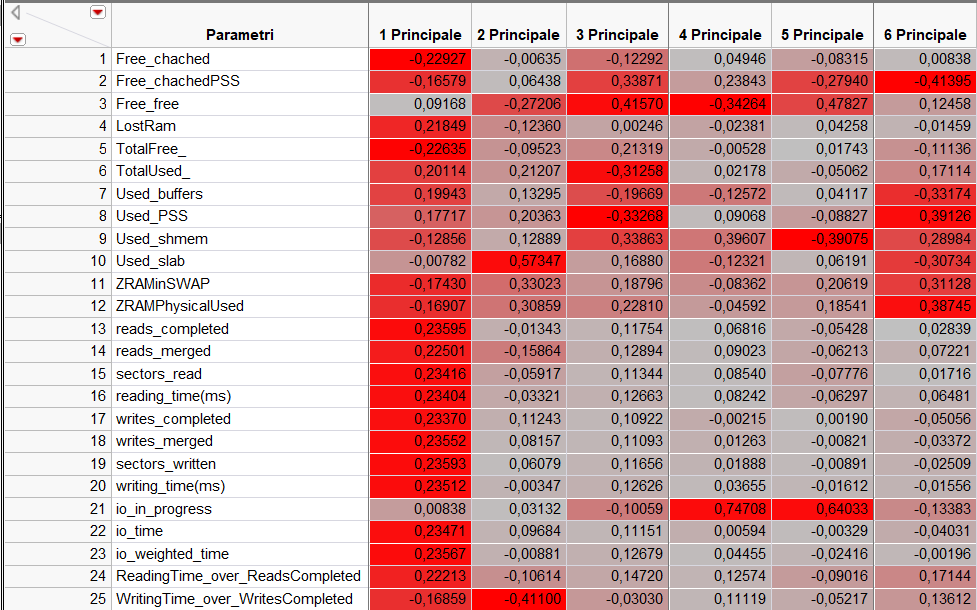
\includegraphics[width=\linewidth,keepaspectratio]{autovettori.png}
  \caption{Autovettori}
  \label{autovettori}
\end{figure}

Nella \figurename~\ref{autovettori} sono evidenziati in rosso i parametri che
hanno contribuito maggiormente, in segno positivo o negativo, alla creazione
delle componenti principali scelte.\\
In particolare:
\begin{itemize}
  \item \textbf{\textit{Principale 1:}} \textit{Free\_chached, LostRam, TotalFree,
  reads\_completed, reads\_merged, sectors\_read, reading\_time(ms),
  writes\_completed, writes\_merged, sector\_written, writing\_time(ms),
  io\_time, io\_weighted\_time e ReadingTime\_over\_ReadsCompleted};
  \item \textbf{\textit{Principale 2:}} \textit{Used\_slab e WritingTime\_over\_WritesCompleted};
  \item \textbf{\textit{Principale 3:}} \textit{Free\_free, TotalUsed e Used\_PSS};
  \item \textbf{\textit{Principale 4:}} \textit{io\_in\_progress};
  \item \textbf{\textit{Principale 5:}} \textit{Used\_shmem};
  \item \textbf{\textit{Principale 6:}} \textit{Free\_chachedPSS, Used\_buffers e Used\_PSS, ZRamPhysicalUsed};
\end{itemize}

\subsection{Clustering}
In questa fase è stato effettuata un'operazione di clustering sul risultato
ottenuto dallo step precedente.\\
La tecnica di clusterizzazione scelta è di tipo gerarchico agglomerativo,
in particolare è stata utilizzata la metrica di \textbf{Ward} per l'aggregazione
dei cluster.\\
In \figurename~\ref{dendogramma} è riportato il dendogramma risultante.\\

\begin{figure}[!htbp]
	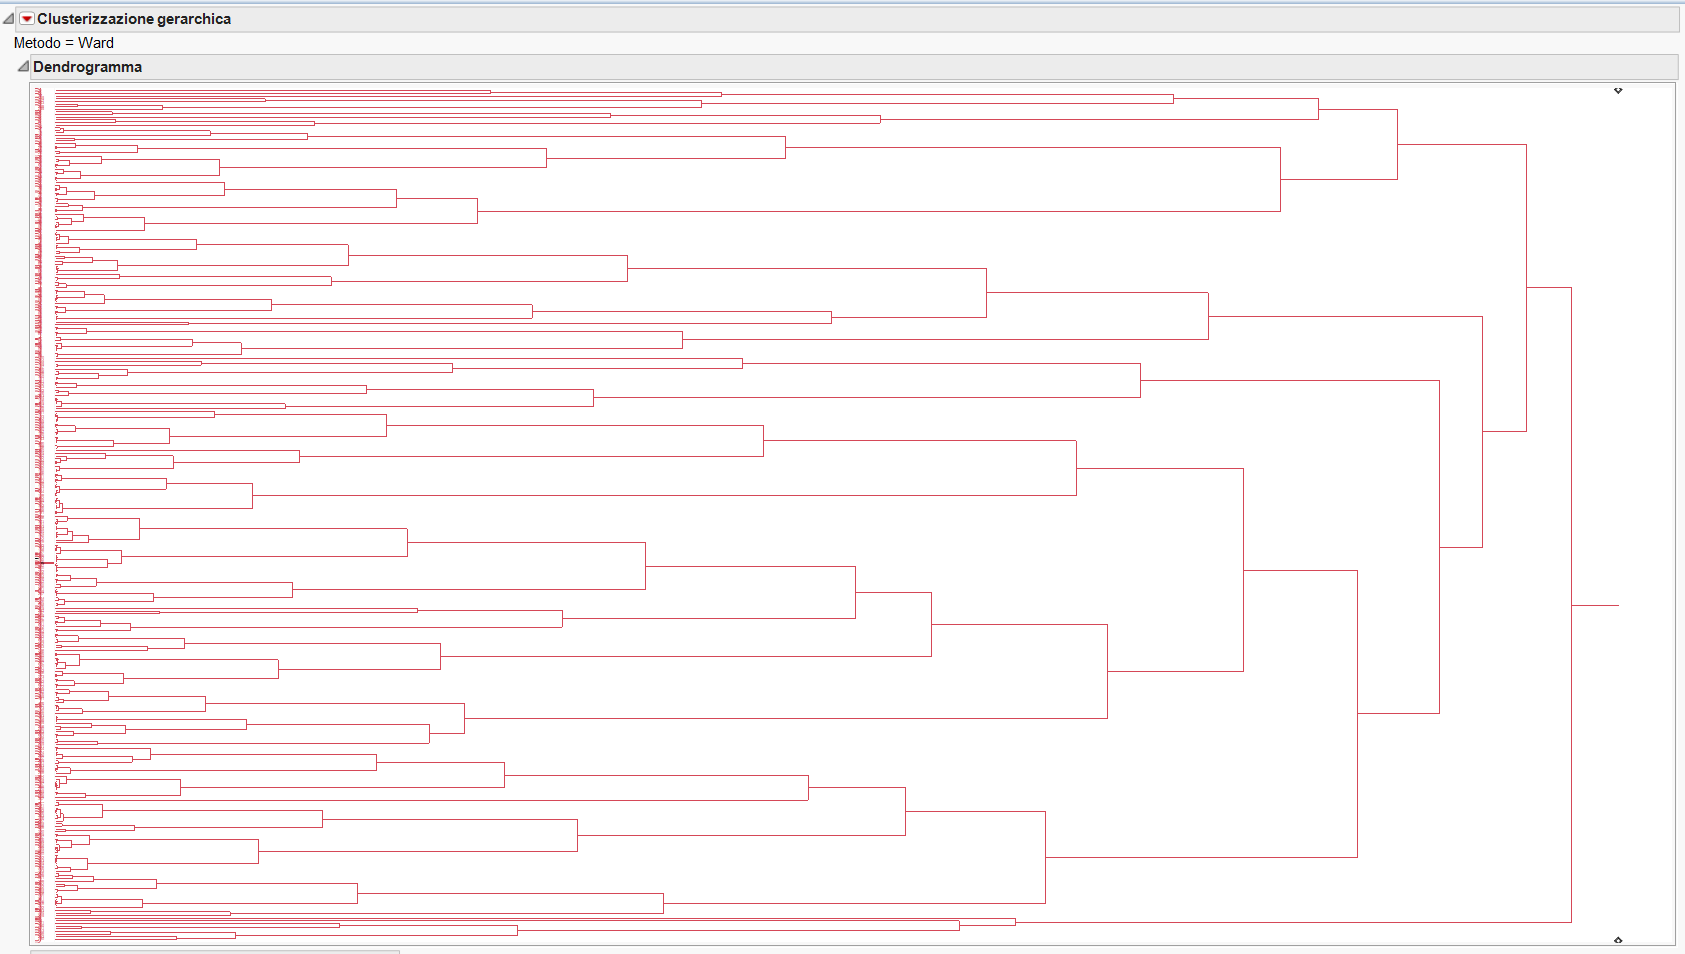
\includegraphics[width=\linewidth,keepaspectratio]{dendogramma.png}
  \caption{Dendogramma}
  \label{dendogramma}
\end{figure}

\begin{figure}[!htbp]
	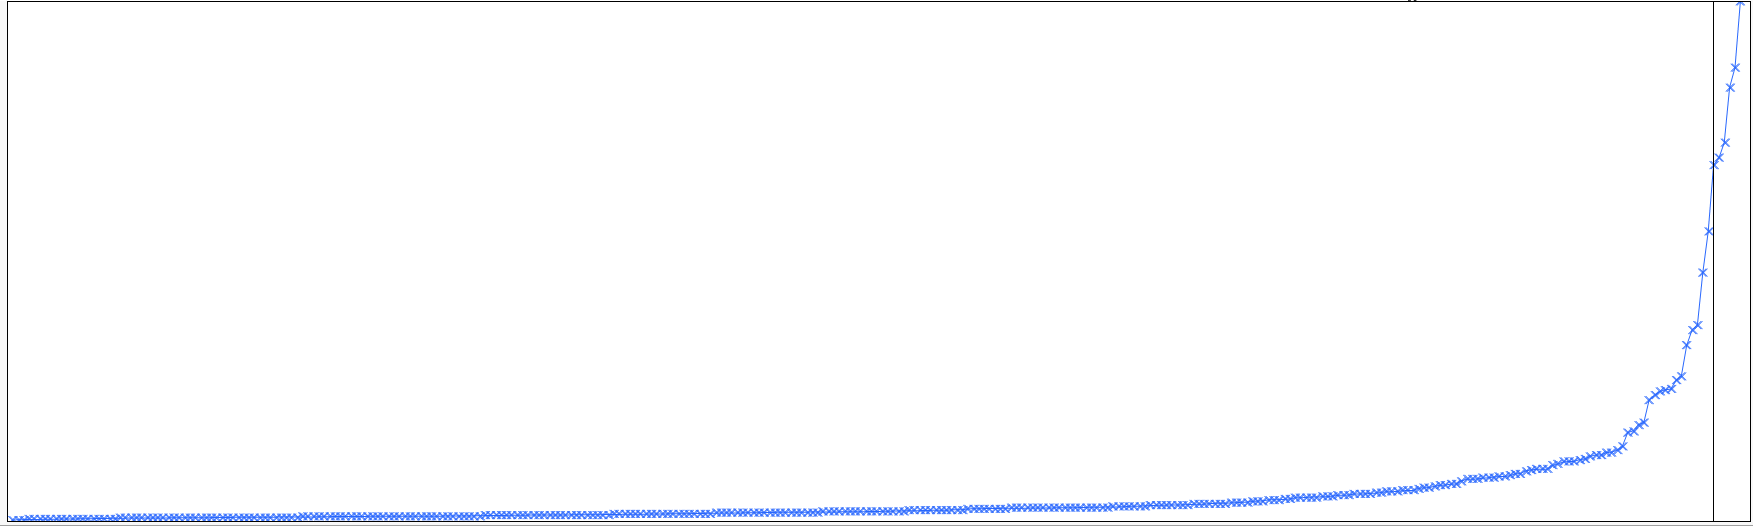
\includegraphics[width=\linewidth,keepaspectratio]{curva_dendogramma.png}
  \caption{Curva di Clustering}
  \label{curva_dendogramma}
\end{figure}

Facendo riferimento alla \figurename~\ref{curva_dendogramma}, si sceglie il numero
di cluster posizionandosi nel ginocchio della curva, rappresentante le distanze tra cluster.\\
\clearpage
In maniera analoga si può scegliere il numero di cluster utilizzando il criterio
di clusterizzazione cubica(\textbf{CCC}), riportato in \figurename~\ref{ccc},
scegliendo il numero di cluster in funzione della regola del massimo salto.\\

\begin{figure}[htbp]
\centering
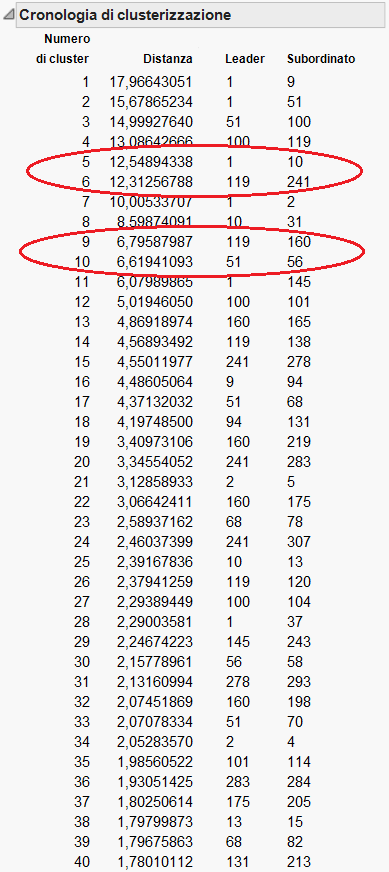
\includegraphics[width=50mm]{gerarchia_clustering.png}% "%" necessario
\qquad\qquad
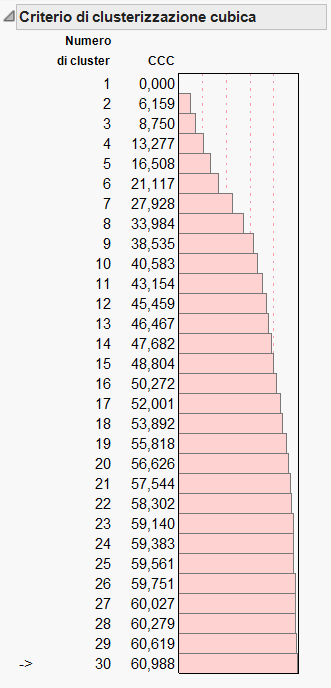
\includegraphics[width=50mm]{ccc.png}
\caption{Gerarchia Clustering e Criterio di Clusterizzazione Cubica}
\label{ccc}
\end{figure}

Sulla base dei criteri illustrati, si è scelto di considerare 6 cluster.\\
Per generare il workload sintetico, inoltre, si è scelto di estrarre ``\textit{Random}''
un esperimento da ogni cluster.\\
\clearpage

\section{Conclusioni}
Ottenuto il Workload Sintetico, è fondamentale osservare quanta varianza si è conservata.\\
Per fare ciò bisogna calcolare la varianza persa in ogni fase del procedimento seguito.\\
A valle della PCA, scegliendo solo 6 componenti principali, la varianza conservata
 risulta essere il 95,702\% della totale(valore ottenuto in JMP).\\
Per definire la significatività del workload ottenuto con il clustering, invece, bisogna
utilizzare la devianza.\\
Quest'ultima è una grandezza indipendente dal grado di libertà, quindi si presta
perfettamente all'uso con i cluster, i quali hanno cardinalità differente.\\

La devianza del clustering è calcolata come la somma della devianza \textbf{inter-cluster}
e \textbf{intra-cluster}.\\
Tipicamente, per effettuare un buon clustering, si cerca di massimizzare la varianza
inter-clustering e minimizzare quella intra-clustering.\\
Nella seguente figura è riportata la devianza del workload sottoposto a PCA.\\

\begin{figure}[!htbp]
	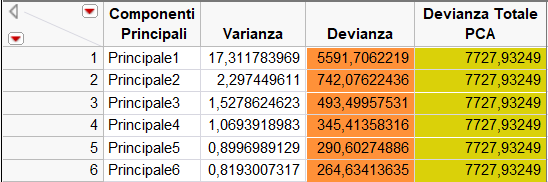
\includegraphics[width=.7\linewidth,keepaspectratio]{devianza_pca.png}
  \caption{Devianza PCA}
  \label{}
\end{figure}
\clearpage

Nella seguente figura è riportata la devianza inter-cluster.\\

\begin{figure}[!htbp]
	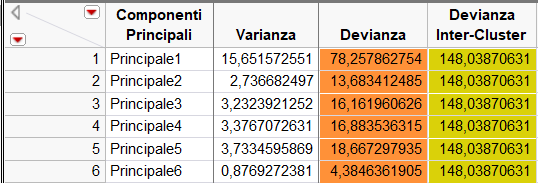
\includegraphics[width=.7\linewidth,keepaspectratio]{devianza_inter_clustering.png}
  \caption{Devianza Inter-Cluster}
  \label{}
\end{figure}

Nella seguente figura è riportata la devianza intra-cluster.\\

\begin{figure}[!htbp]
	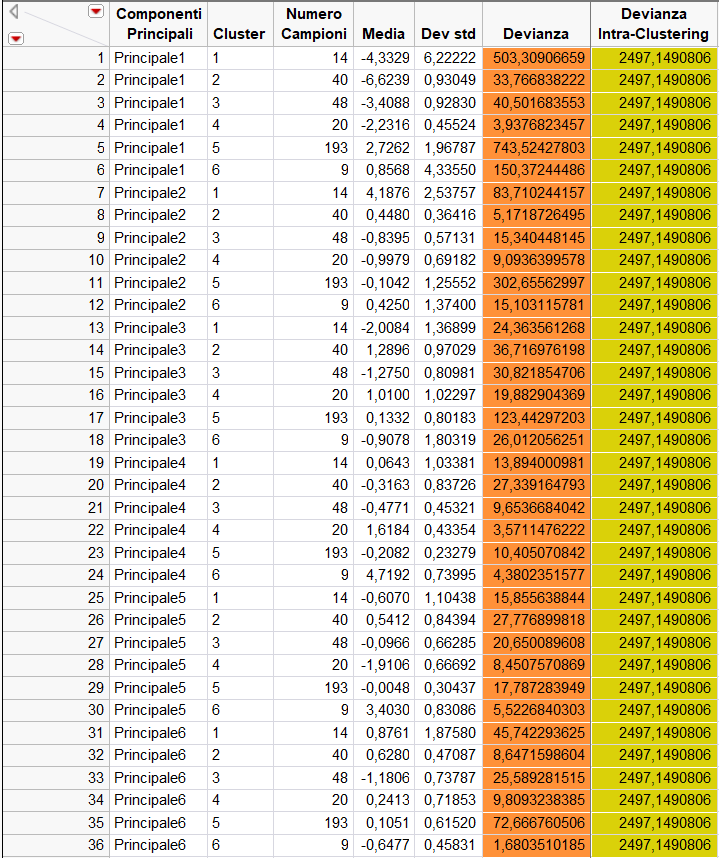
\includegraphics[width=.7\linewidth,keepaspectratio]{devianza_intra_clustering.png}
  \caption{Devianza Intra-Cluster}
  \label{}
\end{figure}
\clearpage

Concludendo, per calcolare la percentuale di devianza conservata utilizzando la
tecnica di clusterizzazione si è utilizzata la seguente formula:
$$1-{devianza_{inter\_cluster}+devianza_{intra\_cluster}\over {devianza_{pca}}}$$

In tabella sono riportate le percentuali di devianza persa e conservata, utilizzando
il clustering.\\

\vspace{5 mm}

\begin{tabular}{|c|c|}
\hline
\textbf{Devianza PCA}	& 7727,93249 \\
\hline
\textbf{Devianza Clustering(intra-cluster+inter-cluster)}	& 2645,1867 \\
\hline
\textbf{Percentuale devianza persa con il clustering}	& 34,22\% \\
\hline
\textbf{Percentuale devianza conservata con il clustering}	& 65,78\% \\
\hline
\textbf{Significatività PCA} &	95,70\% \\
\hline
\end{tabular}

\vspace{5 mm}

In \figurename~\ref{significativita_workload} è riportata la significatività
del workload sintetico.\\

\vspace{5 mm}

\begin{tabular}{c|c|c|}
 & \textbf{Conservata} & \textbf{Perse} \\
 \hline
 \textbf{Workload Reale} & 100,00\% &	0,00\% \\
 \hline
 \textbf{PCA} &	95,70\%	& 4,30\% \\
 \hline
 \textbf{Clustering} &	62,95\%	& 37,05\% \\
 \hline
 \label{significativita_workload}
\end{tabular}

\vspace{5 mm}

In conclusione, utilizzando 6 componenti principali e 6 cluster, si perde il 37,05\%
di significatività rispetto al workload reale.
